\documentclass{article}

\usepackage[utf8]{inputenc} % accents
\usepackage[T1]{fontenc}      % caractères français
\usepackage{geometry}         % marges
\usepackage[francais]{babel}  % langue
\usepackage{graphicx}         % images
\usepackage{verbatim}
\usepackage{url}
\bibliographystyle{alpha}

\title{Document d'analyse des besoins}
\author{Alexandre Casanova-Franger\\
        \and
        Gauthier Lamarque\\
        \and
        Paul Simorre\\
        \and
        Lucas Vivas\\}

\begin{document}
\maketitle
\section{Introduction}
\paragraph{}
Ce projet consiste à améliorer un outil informatique d'analyse sonore dans
l'optique d'approfondir notre compréhension de l'improvisation musicale. À
terme, cet outil aura pour objectif de permettre à des musiciens d'avoir un
aperçu discret (donc quantifié) de leur improvisation. De plus, cet outil aura
une portée scientifique, dans le sens où il sera possible d'étudier l'adaptation
des musiciens grâce aux retours fournis par l'outil. \\
Cet outil est basé sur une plateforme externe appelée Bela \cite{BELA},
qui est un système embarqué de traitement audio en temps réel.
\paragraph{}
À l'origine, six étudiants de l'ENSEIRB-MATMECA ont réalisé un projet similaire
en début d'année 2017, mais ils n'ont pas utilisé le système embarqué Bela. Ils
ont construit un programme en Python, et ont géré les entrées/sorties audio
grâce à des librairies externes. Dans les mois qui suivirent, un de ces six
étudiants, Jérémy Lixandre, a réalisé un stage de deux mois au SCRIME (Studio
de Création et de Recherche en Informatique et Musiques Expérimentales) et a
recommencé le même projet, mais cette fois en se basant sur Bela et son langage
de programmation, le C++. Notre projet est donc la poursuite du travail réalisé
par Jérémy Lixandre durant son stage.
\section{Description et analyse de l'existant}
\paragraph{}
À ce jour, l'outil est capable de fournir une représentation graphique de la
corrélation des entrées audio. La corrélation est une notion centrale
concernant cet outil. La corrélation est en fait une relation statistique
entre deux ou plusieurs variables, et dans notre cas, il s'agit de la
relation entre deux échantillons audio.
\paragraph{}
Les entrées audio sont gérées par le système embarqué Bela, qui peut
recevoir 8 entrées analogiques (par l'intermédiaire de micros), 2 entrées
audio (par l'intermédiaire de prises Jack) et enfin la possibilité d'inclure
des fichiers audio (de type wav).\\
La mécanique principale du programme consiste à récupérer des échantillons
provenant des entrées audio sur un temps donné ($\Delta t$), de les stocker dans
un tableau de vecteur où chaque vecteur (de flottants) représente le signal d'une des entrées.
Ensuite, le programme appliquera sur ces signaux un pré-traitement qui permettra
de modifier les vecteurs afin de pouvoir baser le calcul de corrélation sur différentes
caractéristiques de l'onde. Par exemple, le programme est capable de calculer
l'enveloppe d’énergie d'une onde afin que le calcul de corrélation se fasse en fonction
de cette enveloppe qui permettrait de comparer par exemple les timbres des instruments.
Ensuite il applique une fonction de calcul de corrélation sur chaque paire d'échantillons.
Cette fonction peut changer et permettra de comparer les vecteurs de différentes manière.
\\
Le calcul de la corrélation prend en entrée deux vecteurs de
nombres flottants et renvoie un nombre flottant compris entre 0 et 1.
Dans l'état actuel de l'outil, le calcul de la corrélation correspond au
produit scalaire des deux vecteurs de flottants passés en entrée. Cependant,
grâce au fichier de configuration de l'outil, il est possible de modifier la
méthode de calcul de cette corrélation.\\
Notre prédécesseur devait reconstruire un outil intégralement, et c'est dans
cette optique de simplicité qu'il a fait le choix d'implémenter une version
basique du calcul de corrélation.
\paragraph{}
Enfin, une fois les coefficients de corrélation sont calculés, ceux-ci sont
affichés suivant une matrice de corrélation, où $x_{i,j}$ correspond au
coefficient de corrélation entre l'entrée i et l'entrée j.\\
Sachant cela, la matrice de corrélation obtenue est donc une matrice
symétrique (où $x_{i,j} = x_{j,i}$) et la diagonale de celle-ci est égale à
1 ($x_{i,i} = 1$).
\paragraph{}
Un autre élément central de cet outil est le fichier de configuration
contenant les paramètres nécéssaires au bon fonctionnement du programme. Les
paramètres à renseigner ou à modifier sont les suivants:
\begin{itemize}
	\item L'activation des effets et la taille des buffers correspondants
	      (toutefois, l'ajout d'effets semble diminuer les performances du
	      programme),
	\item Le nombre d'entrées analogiques que l'on souhaite activer (de 0 à 8),
	\item Le nombre d'entrées audio que l'on souhaite activer (de 0 à 2),
	\item Les chemins relatifs vers des fichiers .wav que l'on souhaiterait
	      ajouter en entrée,
	\item Le nom du fichier (sans l'extension \verb!.cpp!) contenant la
	      fonction de conversion du coefficient de corrélation en triplet RGB,
	\item Le nom du fichier (sans l'extension \verb!.cpp!) contenant la
	      fonction de calcul du coefficient de corrélation,
	\item Le nom du fichier (sans l'extension \verb!.cpp!) contenant la
	      fonction de pré-traitement des entrées.
\end{itemize}
\begin{figure}[h]
	\caption{\label{bela_process}Déroulement du programme existant}
	\centering
	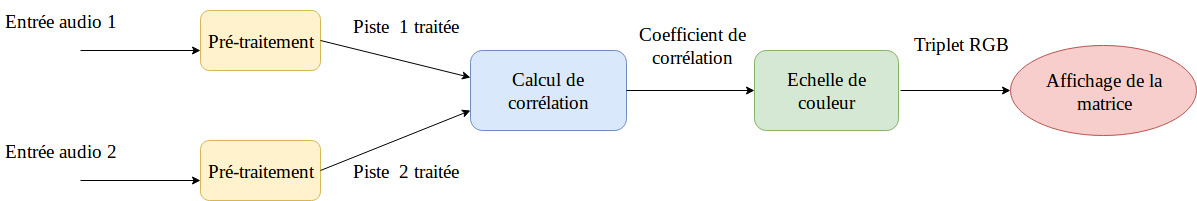
\includegraphics[scale=0.40]{bela_process.jpg}
\end{figure}
\newpage
\section{Description des besoins}
\subsection{Besoins fonctionnels}
\paragraph{}
\begin{itemize}
	\item L'utilisateur pourra avoir un retour sonore, où les volumes des
	      entrées seront modifiés selon un certain mixage (qui dépendra de la
	      corrélation des entrées),
	      \paragraph{}
	      Il s'agit là de l'objectif principal de ce projet. L'utilisateur pourra
	      obtenir un retour audio sur la sortie correspondante du système embarqué.
	      Cependant, les volumes des différentes entrées seront modifiés, il y
	      aura une étape de mixage pour modifier ces volumes, elle sera explicitée
	      lors des prochains points.\\

	\item L'utilisateur pourra choisir une configuration selon laquelle un
	      vecteur de mixage sera créé,
	      \paragraph{}
	      Le mixage sera implémenté comme une fonction qui prendra en entrée la
	      matrice contenant les coefficients de corrélation, et renverra en sortie
	      un vecteur contenant les volumes attribués à chaque entrée.\\

	\item L'utilisateur pourra ajouter une fonction de mixage, qu'il précisera
	      dans le fichier de configuration,
	      \paragraph{}
	      Comme pour les étapes de pré-traitement, de calcul de corrélation, et de
	      conversion vers un triplet RGB, il sera possible pour l'utilisateur de
	      préciser dans le fichier de configuration quel fichier contient la
	      fonction permettant d'obtenir le mixage souhaité. Nous avons évoqué avec
	      les clients différents exemples de mixage, dont les suivants :
	      \begin{itemize}
	      	\item Augmenter le volume des paires d'entrées les plus corrélées,
	      	\item Augmenter le volume des paires d'entrées les moins corrélées,
	      	\item Augmenter le volume des entrées dont la somme des coefficients de
	      	      corrélation avec toutes les autres entrées est la plus élevée.
	      \end{itemize}
	      \paragraph{}

	\item L'utilisateur pourra observer ce vecteur de mixage sur la même page
	      web où figure la matrice contenant les coefficients de corrélation,
	      \paragraph{}
	      Sachant que les utilisateurs de l'outil ne sont pas des développeurs de
	      métier, un affichage graphique reste le meilleur moyen de représenter les
	      informations importantes. La matrice contenant les coefficients de
	      corrélation est représentée par une matrice de carrés colorés, et le
	      code couleur est fourni par une fonction située dans un fichier dont le
	      nom est précisé dans le fichier de configuration. De la même façon, le
	      vecteur de mixage sera représenté par des carrés colorés, et le
	      pourcentage du volume sera indiqué sous ces carrés.\\

	\item L'utilisateur pourra changer les paramètres d'utilisation directement sur
	      l'interface web et non en passant par le fichier de configuration.
	      \paragraph{}
	      Soit tous les paramètres du fichier de configuration qui sont la taille des buffers
	      des échantillons, mettre des effets, et régler le nombre d'entrées analogiques.

	\item l'utilisateur pourra sélectionner la fonction de corrélation temporelle.
	      \paragraph{}
	      Actuellement, l'unique fonction de calcul de corrélation existante est
	      la fonction de corrélation statique qui va calculer un coefficient de corrélation
	      en fonction de tout les points de l’échantillon. Cette nouvelle fonction
	      calculera, à l'aide de transformée de Fourier, le temps ($\tau$) de latence
	      entre deux signaux.


\end{itemize}
\subsection{Besoins non-fonctionnels}
\begin{itemize}
	\item La fonction réalisant le mixage devra être générique.
	      \paragraph{}
	      Comme dit plus haut, il existe déjà trois étapes du programme qui
	      nécessitent des fonctions génériques, et ces fonctions (et leur fichier
	      correspondant) sont précisées dans le fichier de configuration (à
	      modifier avant l'éxécution du programme). De la même manière, la
	      fonction réalisant le mixage des entrées devra respecter les mêmes
	      conditions.
	\item L'ajout d'une fonction de mixage ne devra pas créer de latences.
	      \paragraph{}
	      Dans le rapport émis par le précédent développeur, il est indiqué qu'à
	      partir de 15 entrées, ou avec l'ajout d'effets, des latences sont
	      visibles. Actuellement, le rafraîchissement de la matrice est de l'ordre
	      de la demi-seconde dans son fonctionnement normal. De ce fait, l'étape
	      de calcul du mixage en sortie ne devra pas être trop lourde en terme de
	      temps de calcul, sous peine d'entraîner de fortes latences à l'affichage.
\end{itemize}
\begin{figure}[h]
	\caption{\label{diag_deploiement}Diagramme de déploiement}
	\centering
	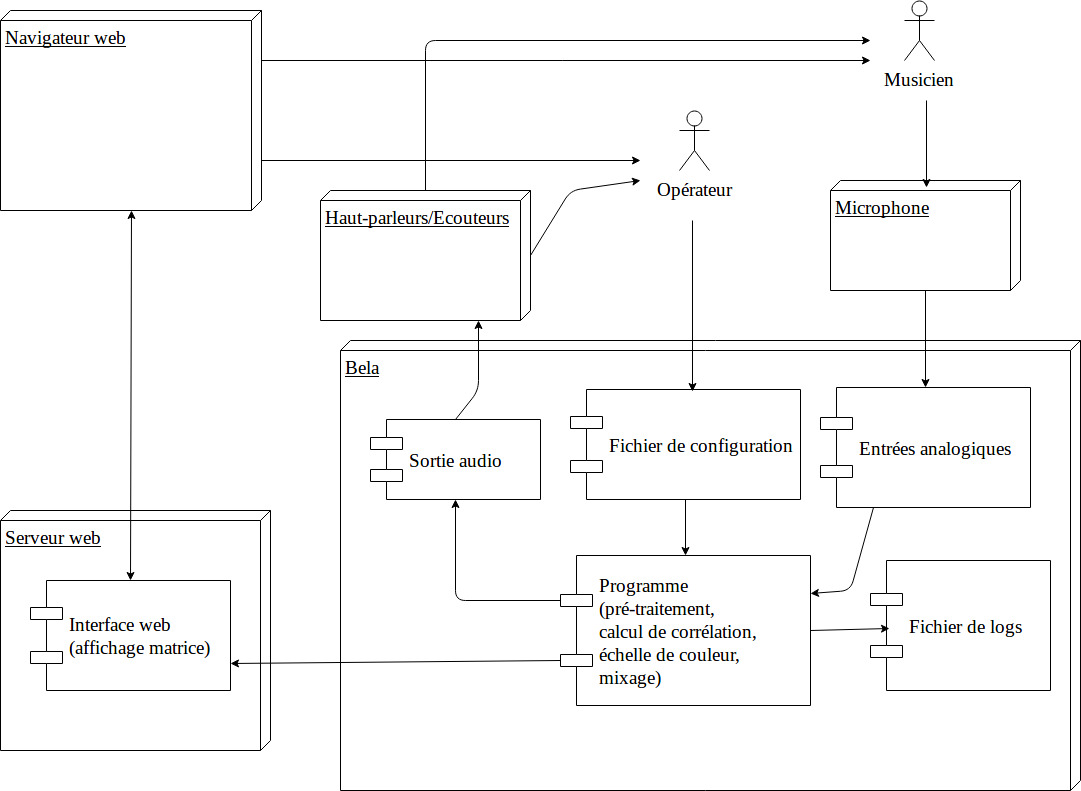
\includegraphics[scale=0.30]{diag_deploiement.jpg}
\end{figure}
\section{Scénario d'utilisation}
\paragraph{}
Nous allons décrire ci-après un scénario d'utilisation. Nous imaginons une
configuration simple pour un scénario réalisable avec une version du projet où
les besoins les plus essentiels aux yeux des clients ont été remplis.
\begin{itemize}
	\item Trois musiciens jouent et s'enregistrent ensemble
	\item Ils veulent obtenir un retour sonore particulier : une version de leur
	      morceau où la paire de musiciens la plus corrélée s'entend plus fort que le
	      troisième musicien
	\item Ils utilisent une version basique du logiciel et l'on suppose donc que
	      les paramètres tels que la fonction de pré-traitement des entrées, la fonction
	      de calcul du coefficient de corrélation et celle calculant sa conversion en
	      triplet RGB auront été choisis par les développeurs
\end{itemize}
Les musiciens improvisent ensemble en tentant de s'accorder les uns avec les
autres. Grâce au dispositif BELA, chaque instrument est enregistré sur une
piste mono-instrumentale isolée. Le logiciel existant traite les données de
leur enregistrement pour fournir la matrice de corrélation ; grâce à ce retour
visuel, le groupe sait déjà quelle paire de musiciens est la plus corrélée à
un instant t donné.
\begin{figure}[h]
	\centering
	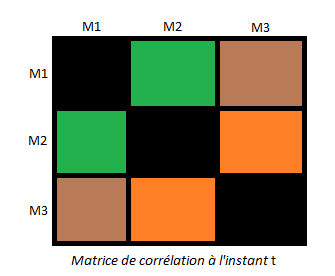
\includegraphics[scale=0.50]{matrice_correlation.png}
\end{figure}
\paragraph{}
Plus la couleur aux indices de deux musiciens est proche du vert clair,
meilleure est la corrélation de leur jeu au moment où cette matrice s'affiche.
On peut voir par exemple qu'à l'instant \textit{t}, les musiciens M1 et M2
sont plus corrélés que les autres couples de musiciens ; ils forment la paire
de musiciens et de pistes mono-instrumentales la plus corrélée.
\paragraph{}
Pour "construire" le retour sonore, notre programme mixe l'enregistrement
grâce aux données de cette matrice. À chaque instant \textit{t}, une valeur
est attribuée à chaque paire de musiciens à partir de son indice de
corrélation. La valeur la plus élevée, celle attribuée à la paire la plus
corrélée, sert à produire un retour sonore sous la forme d'une copie de
l'enregistrement initial où les deux pistes mono-instrumentales constituant
cette paire sont augmentées en volume sonore. Cette paire est donc susceptible
de varier tout au long du morceau : à chaque instant \textit{t}, la paire de
musiciens augmentés en volume sonore peut changer.
\paragraph{}
Les musiciens peuvent alors étudier le retour sonore produit par notre logiciel
et le comparer avec l'enregistrement non modifié par le logiciel. On peut
alors imaginer diverses utilités à ce retour sonore :
\begin{itemize}
	\item Les musiciens pourront préférer conserver l'enregistrement modifié plutôt
	      que l'original
	\item Si deux musiciens sont plus régulièrement augmentés en volume sonore que
	      leur partenaire tout au long du morceau modifié, ce troisième musicien pourra
	      corriger son jeu en conséquence
\end{itemize}


\centering
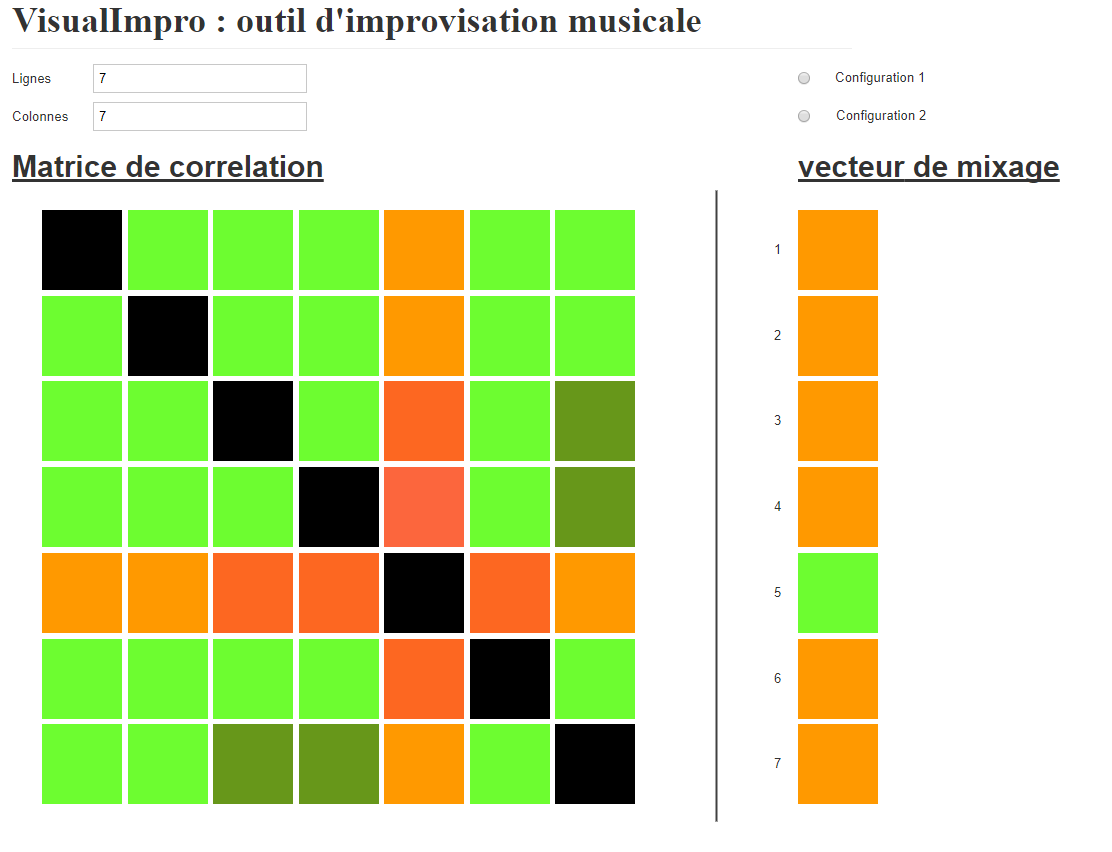
\includegraphics[scale=0.30]{proto_2.png}

\section{Diagramme de Gantt}

\centering
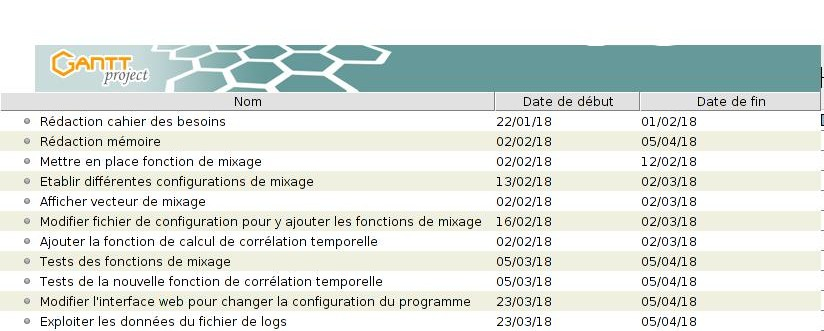
\includegraphics[scale=0.50]{liste_task.jpg}
\centering
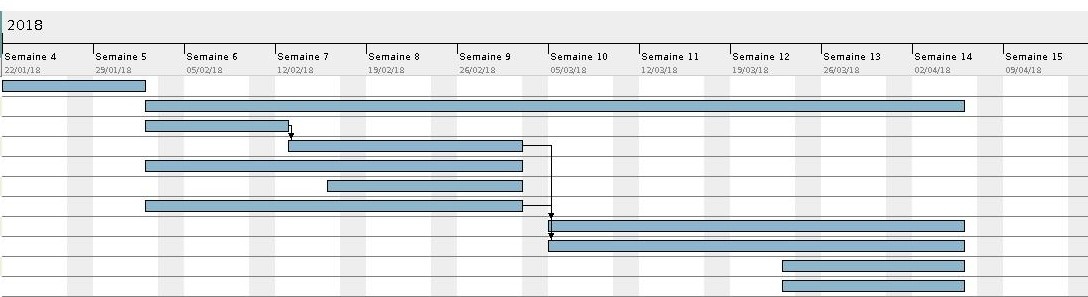
\includegraphics[scale=0.40]{diag_gantt.jpg}

\bibliography{analyse-besoins}
\end{document}
